 \subsubsection{UC11 - Visualizzazione delle informazioni utente}
 \begin{figure}[h]
 	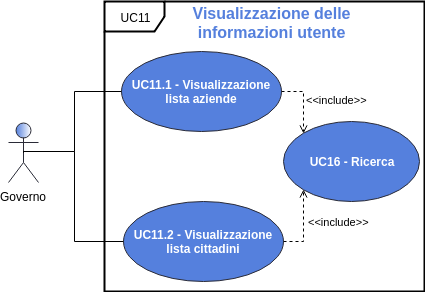
\includegraphics[width=7cm]{res/images/UC11-Generale.png}
 	\centering
 	\caption{UC11 - Visualizzazione delle informazioni utente}
 	
 \end{figure}
 \begin{itemize}
 	\item \textbf{Attori Primari}: governo;
 	\item \textbf{Descrizione}: il governo può accedere alle informazioni riguardanti:
 	\begin{itemize}
 		\item le aziende registrate alla piattaforma;
 		\item i cittadini registrati alla piattaforma.

 	\end{itemize}
 	\item \textbf{Scenario principale}: il governo accede alle informazioni riguardanti gli utenti della piattaforma ed alle eventuali relative operazioni disponibili;

 	\item \textbf{Precondizione}: il sistema riconosce che l'utente è autenticato con privilegi governativi e mostra le pagine utili alla ricerca di informazioni sugli utenti;
 	
 	\item \textbf{Postcondizione}: il governo ottiene dal sistema le liste degli utenti con le eventuali operazioni disponibili.
 \end{itemize}

\subsubsection{UC11.1 - Visualizzazione lista aziende registrate}

 \begin{itemize}
	\item \textbf{Attori Primari}: governo;
	\item \textbf{Descrizione}: il governo visualizza la lista delle aziende registrate alla piattaforma. Per ogni azienda sono rese disponibili le seguenti informazioni:
	\begin{itemize}
		\item chiave\glosp Ethereum\glo;
		\item nome (ragione sociale);
		\item partita IVA;
		\item indirizzo di residenza (sede dell'azienda);
		\item lo stato di "abilitato" o "disabilitato";
		\item indirizzo email;
		\item lo stato del pagamento del saldo IVA, ovvero può controllare se l'azienda risulta:
		\begin{itemize}
			\item \textbf{insolvente}: non ha ancora provveduto alla liquidazione IVA di almeno uno dei trimestri precedenti entro i termini fissati;
			\item \textbf{in fase di pagamento}: l'azienda deve ancora effettuare il versamento IVA riguardante l'ultimo trimestre, ed il termine del pagamento non è ancora scaduto. Nei trimestri antecedenti la situazione risulta "regolare";
			\item \textbf{in dilazione}: in caso l'azienda abbia richiesto il pagamento dilazionato del saldo IVA a debito ed il termine della dilazione non è ancora scaduto;
			\item \textbf{regolare}: l'azienda ha provveduto al pagamento del saldo IVA a debito del trimestre precedente oppure ha ricevuto il rimborso nel caso in cui sia risultata "In attesa di rimborso" nel trimestre precedente;
			\item \textbf{in attesa di rimborso}: nel trimestre precedente il saldo IVA è risultato a credito, e non è ancora stato effettuato il rimborso da parte del governo;
		\end{itemize}
	L'azienda può ricadere in uno solo tra i casi sopra descritti. Lo stato di insolvenza di un trimestre precedente ha la predominanza sugli stati dei trimestri successivi ad esso;
		\item l'importo del saldo IVA.
	\end{itemize}
	
	\item \textbf{Scenario principale}: il governo richiede la lista delle aziende registrate;
	\item \textbf{Inclusioni}:
	\begin{itemize}
		\item \textbf{UC16}: l'utente può filtrare i risultati visualizzati inserendo una parola chiave.
	\end{itemize}
	\item \textbf{Precondizione}: il sistema riconosce che l'utente è autenticato con privilegi governativi ed ha richiesto di ottenere la lista di tutte aziende;
	\item \textbf{Postcondizione}: il governo ottiene dal sistema la lista delle aziende registrate, con associate le operazioni che può effettuare su di esse.
\end{itemize}

\subsubsection{UC11.1.1 - Visualizzazione filtrata lista aziende registrate}
\begin{figure}[H]
	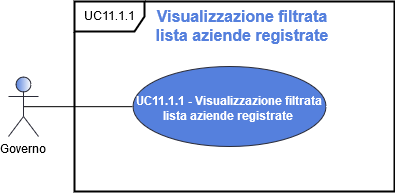
\includegraphics[width=7cm]{res/images/UC11-VisualizzazioneFiltrata.png}
	\centering
	\caption{UC11 - Visualizzazione filtrata lista aziende registrate}
\end{figure}
\begin{itemize}
	\item \textbf{Attori Primari}: governo;
	\item \textbf{Descrizione}: il governo visualizza la lista delle aziende registrate alla piattaforma, filtrate secondo il valore del campo \texttt{stato del pagamento del saldo IVA}. I possibili valori per filtrare i risultati per tale campo sono i seguenti:
	\begin{itemize}
		\item insolvente;
		\item in fase di pagamento;
		\item in dilazione
		\item regolare;
		\item in attesa di rimborso.
	\end{itemize}
	
	\item \textbf{Scenario principale}: il governo filtra le aziende visualizzate secondo il valore del campo \texttt{stato del pagamento del saldo IVA}. Seleziona tale valore servendosi dell'apposito menù a tendina;
	\item \textbf{Precondizione}: l'utente governativo ha eseguito l'accesso alla pagina dedicata alla visualizzazione delle aziende registrate, ed ha selezionato un'opzione per filtrare le aziende;
	\item \textbf{Postcondizione}: il governo ottiene dal sistema la lista delle aziende registrate, filtrate a seconda del valore del campo \texttt{stato del pagamento del saldo IVA} selezionato.
\end{itemize}


\subsubsection{UC11.2 - Visualizzazione lista cittadini}
\begin{itemize}
	\item \textbf{Attori Primari}: governo;
	\item \textbf{Descrizione}: il governo ottiene la lista dei cittadini. Per ognuno di essi può visualizzare:
	\begin{itemize}
		\item la chiave\glosp Ethereum\glo;
		\item il nome;
		\item il cognome;
		\item l'indirizzo di residenza;
		\item indirizzo email.
	\end{itemize}
	\item \textbf{Scenario principale}: il governo richiede la lista dei cittadini. Per ognuno di essi visualizza le rispettive informazioni;
	\item \textbf{Inclusioni}:
	\begin{itemize}
		\item \textbf{UC16}: l'utente può filtrare i risultati visualizzati inserendo una parola chiave.
	\end{itemize}
	\item \textbf{Precondizione}: il sistema riconosce che l'utente è autenticato con privilegi governativi ed ha richiesto di ottenere la lista di tutti i cittadini;
	\item \textbf{Postcondizione}: il governo ottiene dal sistema la lista dei cittadini, con associate le operazioni che può effettuare su di essi.
\end{itemize}


